\documentclass{report}
\usepackage{float}

% depricated
\title{
	\iffalse
	\begin{tikzpicture}[remember picture,overlay]
		\node[anchor=north west,yshift=-5pt,xshift=-200pt]%
		at (current page.north east)
		{
\includegraphics[height=30mm]{unitn-logo}};
	\end{tikzpicture}
	\huge 
	\fi
	FixMi \\
	Analisi dei Requisiti
}
\author{Giovanni Santini, Riginel Ungureanu, Valerio Asaro}
\date{Anno accademico 2023/2024}

% for the image in the title
\usepackage{tikz}

% custom spacing
\usepackage{setspace}
\onehalfspacing

% footer and header
\usepackage{fancyhdr}
% \setlength{\headheight}{15.2pt}

% Table of contents link to corresponding sections
\usepackage{hyperref}
\hypersetup{
	colorlinks,
	citecolor=black,
	filecolor=black,
	linkcolor=black,
	urlcolor=black
}

% Remove che "Chapter" string before chapters
\iffalse
\makeatletter
\def\@makechapterhead#1{%
	\vspace*{50\p@}%
	{\parindent \z@ \raggedright \normalfont
		\interlinepenalty\@M
		\Huge\bfseries  \thechapter.\quad #1\par\nobreak
		\vskip 40\p@
}}
\makeatother
\fi

% Fancy chapters
\usepackage[Bjarne]{fncychap}
% options: Sonny, Lenny, Glenn, Conny, Rejne, Bjarne, Bjornstrup

\begin{document}
	
	
	%title page
	\begin{titlepage}
		\begin{figure}[t]
			\centering
\includegraphics[width=0.3\textwidth]{unitn-logo}
		\end{figure}
		\begin{center}
			\textsc{ \LARGE{Università degli Studi di Trento \\}}
			\textsc{ \LARGE{Facoltà di Informatica\\ }}
			\textnormal{ \LARGE{Corso di Ingegneria del Software\\}}
			\vspace{30mm}
			\fontsize{10mm}{7mm}\selectfont 
			\textup{FixMi \\ Specifica dei Requisiti}\\
		\end{center}
		
		\vspace{25mm}
		
		\centering
		\large Giovanni Santini\\ Riginel Ungureanu \\ Valerio Asaro
		
		\vspace{20mm}
		
		\centering{\large{Anno Accademico 2023/2024 \\ Trento }}
		
	\end{titlepage}
	
	
	
	
	% use header and footers
	\pagestyle{fancy}
	\fancyhead[R]{\chaptername\ \thechapter}  % header
	
	%\maketitle
	\tableofcontents
	\newpage
	
	
	
	\section{Scopo del documento}
	
	Nel presente documento vengono riportate le specifiche dei requisiti di sistema del progetto FixMi,  attraverso diagrammi di tipo Unified Modeling Language (UML) e tabelle strutturate.\\
	
	
	
	\section{Informazioni del Documento}
	
	% table
	\begin{center} % center the table
		\centering
		\begin{tabular}{ |p{4cm}|p{4cm}|  }
			\hline
			\centering Campo & \qquad\qquad Valore \\ % I found no other way...
			\hline
			Titolo del Documento & Specifica dei Reqiusiti \\
			\hline
			Titolo del Progetto & FixMe \\
			\hline
			Autori del Documento &
			Giovanni Santini \\ & Riginel Ungureanu \\ & Valerio Asaro \\
			\hline
			Project Manager & Riginel Ungureanu\\
			\hline
			Versione del documento & 1.0 \\
			\hline
		\end{tabular}
	\end{center}


\chapter{Requisiti}

	
\section{Requisiti Funzionali}

TODO: Qui per ogni requisito funzionale del D1 dobbiamo fare uno o più diagrammi in base all'esigenza tra i seguenti:
\begin{itemize}
	\item Use Case Diagram: Visione esterna del sistema
	\item Sequence Diagram: Rappresenta come gli oggetti collaborano
	\item State Machine Diagram: Stati e Transizioni
	\item Activity Diagram: Attività che triggano altre (tasks)
	\item Spiegazione in italiano (da mettere sempre)
\end{itemize}

\subsection*{RF1 Login }
\begin{figure}[H]
	\centering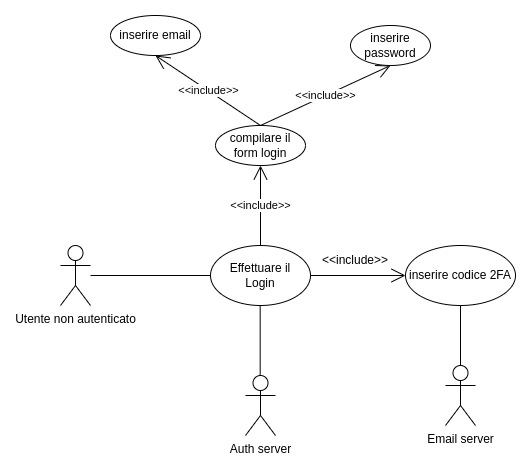
\includegraphics[width=1\textwidth]{images/Login_UCD.drawio.png}
	Use Case Diagram  del login
\end{figure}
Per descrivere questo use case, facciamo uso di un diagramma delle attività swimlane:
\begin{figure}[H]
	\centering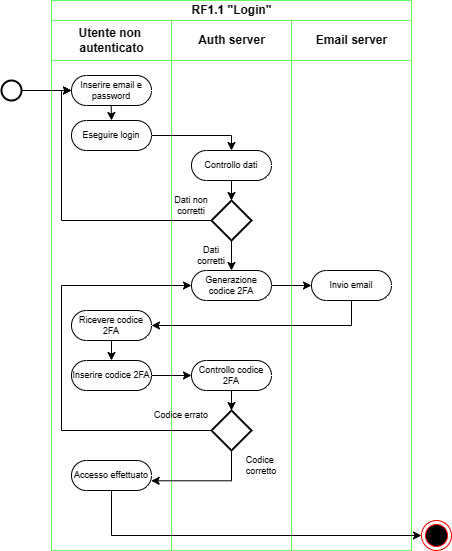
\includegraphics[width=1\textwidth]{images/Login_Swimlane.drawio.png}
	diagramma delle Attività swimlane del Login
\end{figure}
\subsection*{RF2 Registrazione}
\begin{figure}[H]
	\centering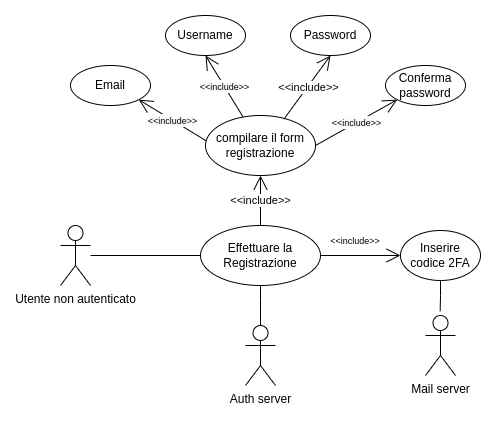
\includegraphics[width=1\textwidth]{images/Registrazione_UCD.drawio.png}
	Use Case Diagram  della registrazione
\end{figure}
Per descrivere questo use case, facciamo uso di un diagramma delle attività swimlane:
\begin{figure}[H]
	\centering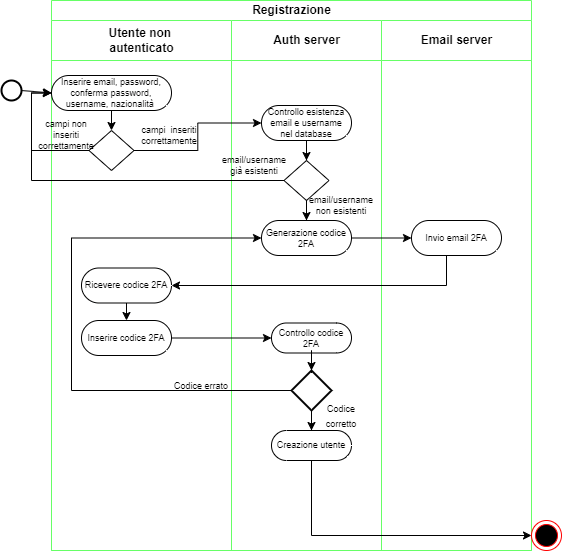
\includegraphics[width=1\textwidth]{images/Register_swimlane.drawio.png}
	diagramma delle Attività swimlane della registrazione
\end{figure}

\subsection*{RF3 Negozio utente non autenticato + RF5 Negozio utente autenticato}

\begin{figure}[H]
	\centering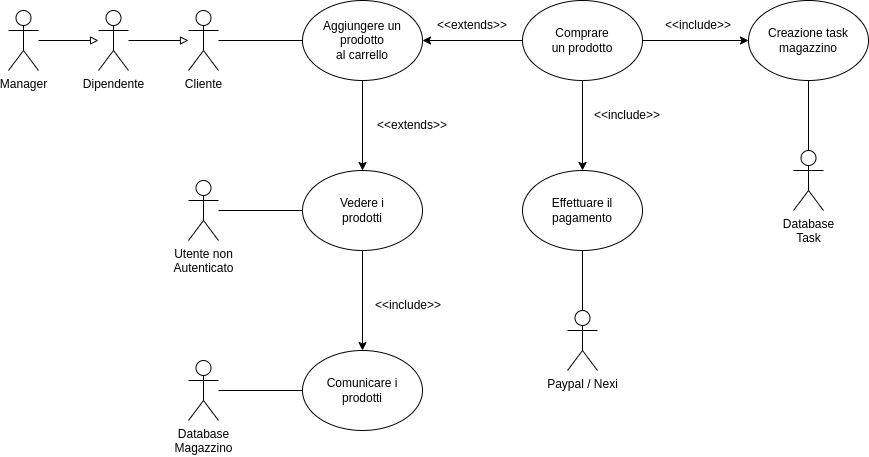
\includegraphics[width=1\textwidth]{images/shop_diagram_1.png}
\end{figure}

\begin{figure}[H]
	\centering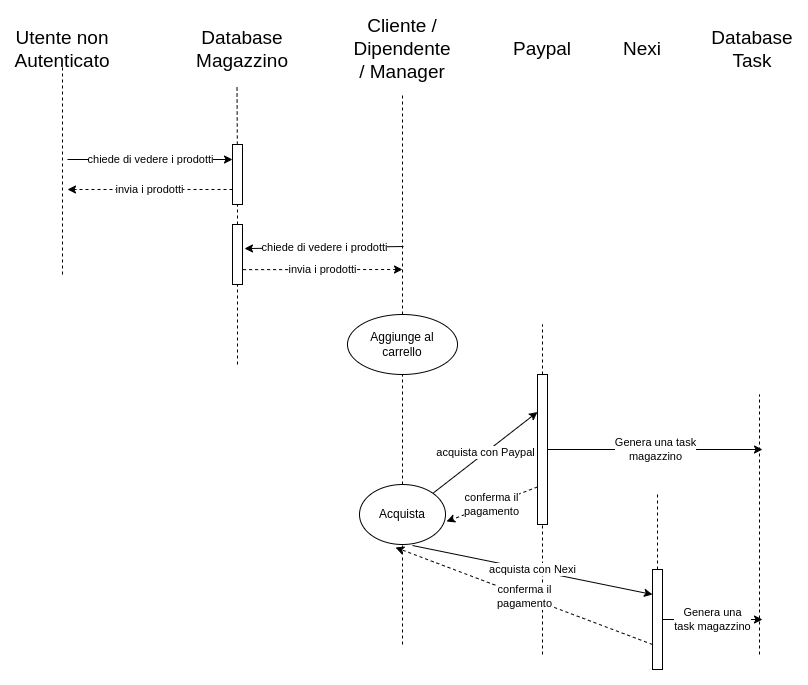
\includegraphics[width=1\textwidth]{images/negozio_sequence_diagram.png}
	diagramma delle Attività swimlane della registrazione
\end{figure}

\subsection*{RF6 Riparazione}

\subsection*{RF7 Assistenza}

\subsection*{RF8 Feedback}

\subsection*{RF9 Tasks}

\subsection*{RF10 Magazzino}

\subsection*{RF11 Gestione Dipendentio}

\pagebreak

\section{Requisiti Non Funzionali}

TODO: Gli stessi del D1 ma messi in una tabella + unità di misura di ogni requisito

\subsection*{RNF1 Intuitività e Accessibilità}
% table
\begin{center} % center the table
	\centering
	\begin{tabular}{ |p{3cm}|p{4cm}|p{4cm}|  }
		\hline
		\centering Proprietà & \qquad\quad Descrizione & \qquad\qquad Misura\\ % I found no other way...
		\hline
		Linguaggio Comprensibile & In media l’utente deve essere in grado di capire le funzionalità dell'applicazione con una
		sola lettura della descrizione &  \\
		\hline
	\end{tabular}
\end{center}

\subsection*{RNF2 Sicurezza}
\subsection*{RNF3 Privacy}
\subsection*{RNF4 Affidabilità e Disponibilità}
\subsection*{RNF5 Performante}
\subsection*{RNF6 Compatibilità e Portabilità}
\subsection*{RNF7 Mantenibilità e Scalabilità}
\subsection*{RNF8 Conformità}

\chapter{Analisi del Constesto}

\section{Utenti e Sistemi Esterni}

TODO: Enumerare gli Utenti e Sistemi Esterni


\section{Diagramma di Contesto}

Spiegare la back-end andando su vari livelli di dettaglio:
\begin{itemize}
	\item Context diagram generale
	\item Divisione in processi
	\item Divisione in Sub Processi
	\item Data flow diagram per i processi (e i sub processi se siamo bravi)
\end{itemize}
\chapter{Analisi dei Componenti}

\section{Definizione dei Componenti}

Componenti interni della mia applicazione e come interagiscono\\
Sostanzialmente sono i componenti usati nei RF in questo documento

\section{Diagramma dei Componenti}

\end{document}